\documentclass[10pt]{article}
\usepackage[usenames]{color} %used for font color
\usepackage{amssymb} %maths
\usepackage{amsmath} %maths
\usepackage[utf8]{inputenc} %useful to type directly diacritic characters
\usepackage[letterpaper, portrait, margin=1.5in]{geometry}
\usepackage{multicol}
\usepackage{graphicx,wrapfig}
\usepackage{hyperref}
\begin{document}
\subsection*{MSDS600 Week 7 Assignment - Nathan Worsham}
\begin{figure}[!h]
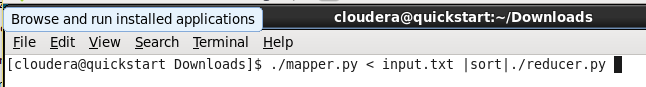
\includegraphics[scale=0.5]{reducer_command.png}
\centering
\end{figure}
\noindent I worked through the instructions for this assignment running the python code as is: \\*
\begin{figure}[!h]
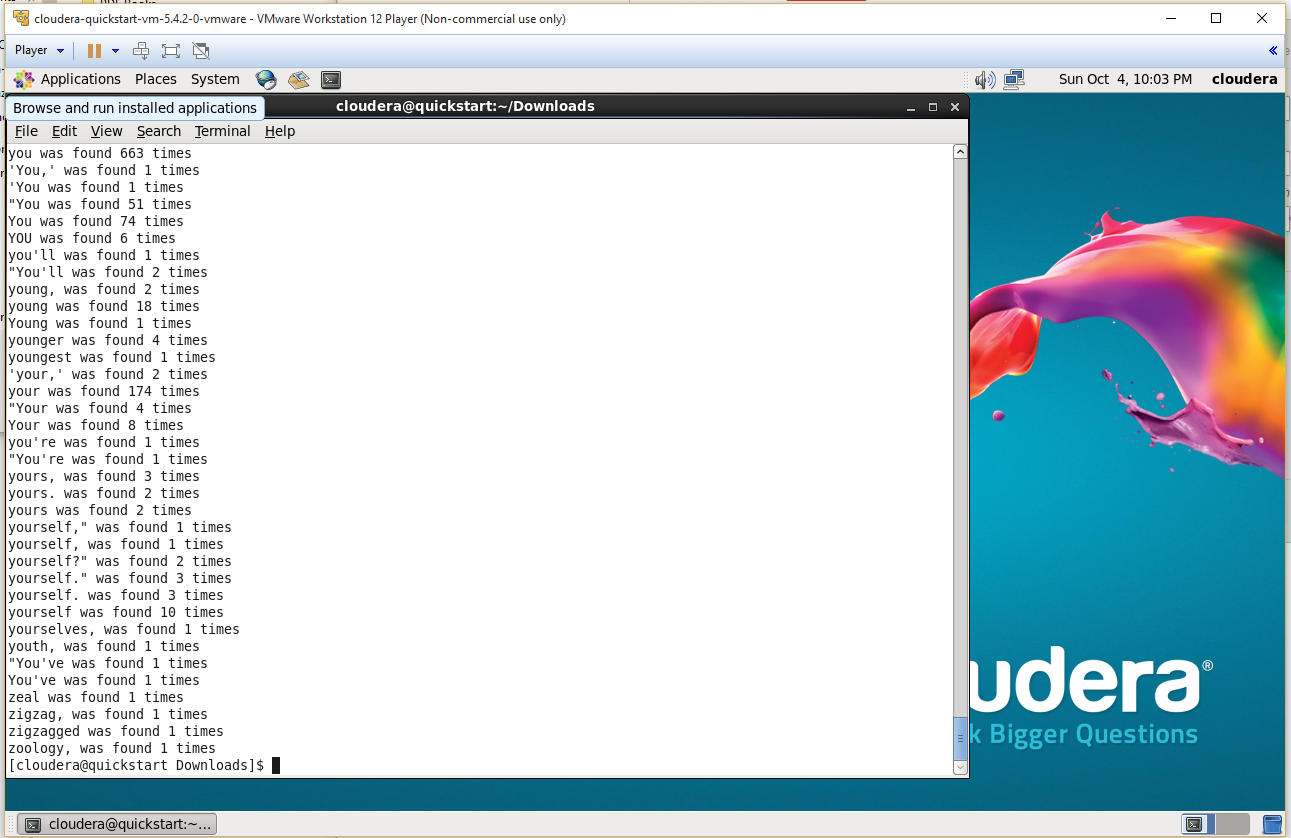
\includegraphics[scale=0.3]{reducer_results.png}
\centering
\end{figure}\\*
\noindent I ran into just a couple of minor issues. The first was getting the files to the VM machine. I ended up using the built-in Firefox browser to go to the worldclass.regis.edu site to get the files. The other issue I ran into is that the files were not executable, so for the files that needed to be executable—mapper and reduce—I ran the command: 
\begin{verbatim}
chmod 755 filename 
\end{verbatim}
Next, I was having trouble understanding what the assignment wanted us to accomplish. I do not really know how to write any Java code so I started by Googling for a “Hadoop Python SDK”. This brought me to a blog post on Cloudera’s site called “A Guide to Python Frameworks for Hadoop” by Uri Laserson (2013). In this post it had a section on Hadoop Streaming, which from the reading I had learned that the streaming API allows non-Java programing languages to be used to interact with the Hadoop system. The example python scripts on the site were even named the same—mapper.py and reducer.py—so I felt this was the right route to go and where I spent my time trying to get to work. Later I learned that really just running the python scripts was the assignment, but I did not feel that gave me any understanding on how to use Hadoop as the supplied scripts were really just running some already written python code piped through a bash command and piped again to another python script.  
Since the Cloudera example uses a mapper and reducer script and I was already given similar python files, I mostly concentrated on the example they gave to execute the command:\pagebreak
\begin{figure}[!h]
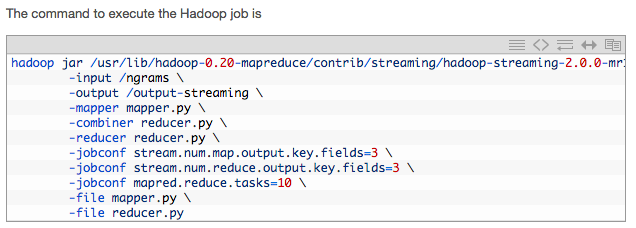
\includegraphics[scale=0.5]{week7_hadoop_example_command.png}
\centering
\end{figure}\\*
I realized that my reducer.py file would need to be edited to produce a different output as their reducer script example gave a tab separated output. I copied the output line, commented out the original and changed it so that it just outputted a key and value separated by a tab: 
\begin{verbatim}
#print previous_key+" was found "+str(total)+" times" 
print previous_key+"\t"+str(total) 
\end{verbatim}
Trying to run roughly the same command minus the key field settings because in their example the key had tabs in it. I quickly found that some of these options they showed were old or deprecated options from the help file that appeared on the screen because I ran the command incorrectly. Instead of having to specify each script on its own option (\verb|-file|), the new option was \verb|-files| and you give it a comma separated list, and the new option has to go at the beginning of the command. The help file mentioned that this option was so that each node gets the script and can execute it. Next I found that the \verb|-jobconf| option was deprecated, the example was trying to use this to set the number of reduce tasks, I found the option \verb|-numReduceTasks| instead. 
\begin{figure}[!h]
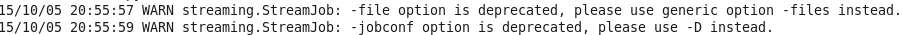
\includegraphics[scale=0.55]{failed_streaming.png}
\centering
\end{figure}\\*
Now that I had my command correct I was still getting errors that it could not find my inputs.txt file as it was giving me an error about “input path does not exist". I was very confused here as I wasn’t sure how to get it my file (I tried giving it a fully qualified path and placing the file in the home directory of the user to no avail). Stackoverflow.com to the rescue! In the post I found, I realized that you treat the Hadoop file system almost as if it were a web or ftp site, you have to upload your input file to it using the \verb|hadoop fs| command. So I then used \verb|hadoop fs -put input.txt| to upload my input file. Now my command finally started to work:\pagebreak
\begin{figure}[!h]
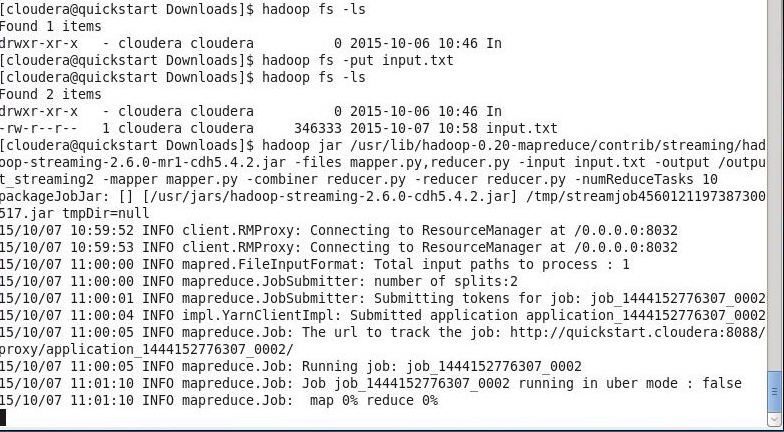
\includegraphics[scale=0.45]{cloudera_start1.jpg}
\centering
\end{figure}\\*
I suppose I was surprised how long it took to run the MapReduce job. I know that this is running on a VM which would cause performance issues but in "real life" I work with a product called Splunk which also uses the concept of MapReduce, and on Splunk no matter if you are on a single node or many the operation to ingest (and retrieve) data is nearly realtime. Last I wanted a way to check that my data was truly in the HDFS. I was able to find that the same \verb|fs| command allows you to "cat" (which actually stands for concatenate) a file or group of files. So using \verb|hadoop fs -cat /output_streaming/*| I was able to see my results which looked very similar to the output of the python script example:
\begin{figure}[!h]
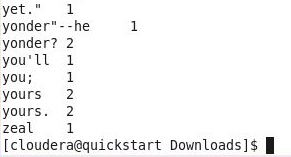
\includegraphics[scale=0.8]{cloudera_catoutput1.png}
\centering
\end{figure}\\*
\pagebreak
\subsection*{References}
Laserson, Uri, 2013. A Guide to Python Frameworks for Hadoop. Retrieved from\\*
http://blog.cloudera.com/blog/2013/01/a-guide-to-python-frameworks-for-hadoop/\\*
Stackoverlow.com, 2013. Retrieved from http://stackoverflow.com/questions/15191832/first-hadoop-project-error-input-path-does-not-exist
\end{document}